

\documentclass[UTF8]{ctexart}

\title{\heiti 杂谈勾股定理}
\author{\kaishu 张三}
\date{\today}
\bibliographystyle{plain}
\newtheorem{thm}{定理}
\usepackage{graphicx}
\usepackage{float}
\usepackage{amsmath} % 用来引用公式相关。\eqref{label} 命令就可以使用。
\usepackage{geometry}%几何结构。负责页面布局。
	\geometry{a6paper,centering,scale=0.8}%a6大小,版面中心,长款占页面0.8
	
%将表格,参考文献加入目录的方法,使用tocbibind 宏包。
\usepackage[nottoc]{tocbibind} %默认加入目录项本身,参考文献,索引等项目。
%nottoc 取消目录本身的显示。

% 我们可以看到图标的标题如果太长的话,标题的下一行会与 图 字对齐,这里我们需要设置成悬挂对对齐的方式。使用caption宏包,来设定标题格式。
\usepackage[format=hang, font = small, textfont=it]{caption} %hang,表示悬挂。
% font表示字号。 textfont = it 表示斜体。italic 表示斜体。对汉字来说就是楷书。

%至于题目,作者,时间等设置,则只需要在其本身命令中设置参数即可。
\newenvironment{myquote}
	{\begin{quote}\kaishu\zihao{-5}}
	{\end{quote}}

%数学公式的右上角的角度符号也可以用 newcommand 来重新定义。
\newcommand{\degree}{^\circ}

\begin{document}
	\maketitle
	\begin{abstract}
		\centering
		这是一篇关于勾股定理的小短文。
	\end{abstract}
	\tableofcontents
	\section{勾股定理在古代}\label{sec:gudai}
	在中国,商朝时bai期的商高提出了“勾三股四玄五”的勾股定理的特例。zhi在西方,最早提出并证明此定理的为dao公元前6世纪古希腊的\cite{quanjing}毕达哥拉斯学派\footnote{欧几里得,约公元前 330--275 年。},他用演绎法证明了直角三角形斜边平方等于两直角边平方之和。毕达哥拉斯学派么有书面著作,该定理的严格表述和证明则监狱欧几里得《几何原本》的命题47:‘直角三角形的斜边上正方形等于量两个正方形之和。’证明是用面积做的。

	我国的周髀算经在商高达州公约(约公元前12世纪) 答周公约:
%	\begin{quote}
%		\zihao{-5}\kaishu 狗广三,故修斯,进购物。
%%	\end{quote} 这种引用的方法,引用里边还有很多命令,看起来是十分不便利的,我们可以自己构建新的环境来进行设置。 \newenvironment{name}{begdef}{enddef} name:新环境的名字,begdef :环境开始的代码,enddef :环境结束的代码。
	\begin{myquote}
		勾广三,股修四,径偶五。
	\end{myquote}
	又载陈子大荣:
%	\begin{quote}
%		\zihao{-5}\kaishu 若求邪至日者,以日下为句,日高为股,句股各自乘,并而开方除之,得邪至日。
%	\end{quote}

	\begin{myquote}
		若求邪至日者,以日下为句,日高为股,句股各自乘,并而开方除之,得邪至日。
	\end{myquote}
	
	图\ref{fig:xiantu} 就是我国古代的一种证明。
	\begin{figure}[ht]
		\centering
		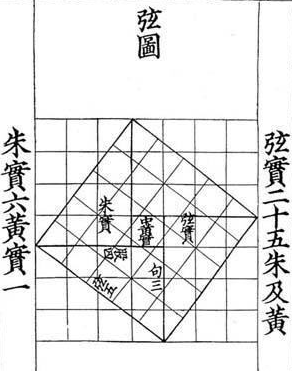
\includegraphics[width=3cm]{zhoubi.png}
		\caption{\kaishu 宋赵爽在《周髀算经》注中做的玄图,该图给出了勾股定理的一个极具对称美的证明。}
		\label{fig:xiantu}
	\end{figure}
	%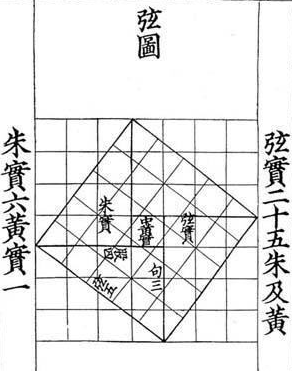
\includegraphics[width=3cm]{zhoubi.png}
	
	\section{勾股定理在近代的形式}
	勾股定理可以用现代语言表示如下:
	\begin{thm}[勾股定理]
		直角三角形斜边的平方等于两腰的平方和。
		
%		可以用符号语言表是为:设直角三角形ABC,其中$\angle C = 90^{\circ}$, 则有
可以用符号语言表是为:设直角三角形ABC,其中$\angle C = 90\degree$, 则有
		\begin{equation}
			AB^2 = BC^2+AC^2 \label{eq-gougu}
		\end{equation} 
	\end{thm}	
	
	\begin{equation}\label{eq:gougu}
		ab^2+bc^2=ac^2
	\end{equation}
	
	满足式(\ref{eq-gougu})的整数称为\emph{勾股数}。第\ref{sec:gudai}%引用第一节。
	节所说的毕达哥拉斯学派得到的三元数组就是勾股数,满足式\eqref{eq:gougu}也成为勾股数。下表列出一些较小的勾股数:
	%可以看出两种引用和公式的方式,第二种直接是自动添加了括号。
	\begin{table}[H] %连贯,使得表格不浮动,需要用float宏包。
		\centering
		\begin{tabular}{|r r r|}
			\hline
			直角边a & 直角边b & 斜边c\\
			\hline
			3 &4 & 5 \\
			5 & 12 & 13 \\
			\hline
		\end{tabular}%
		\qquad  %2em 一个em大约M的宽度。
		($a^2+b^2=c^2$)
		\caption{}
		\label{fig:1}
	\end{table}
		
		

	
	\nocite{Shiye}
	\bibliography{math} %参考文献的数据库。
	
\end{document}